%tag:0007
%label:"art:heegaardFloerExposition"
%author:JeffHicks
%name:"a sketch of Heegaard-Floer theory"
%type:"exposition"
%source:"ozsvath2004introduction"


We have a complete classification of surfaces; we can effectively ``draw'' all oriented surfaces. The proof of the classification of surfaces can be stated in terms of \emph{fundamental polygons}:
\begin{itemize}
    \item First, one shows that every surface can be represented by a polygon with edge identifications, 
    \item Then, one shows that there are several ``moves'' on fundamental polygons that modify the combinatorial data of the fundamental polygon but correspond to the same surface,
\end{itemize} 
%label:"fig:fundamentalPolygonsT2"
%author:JeffHicks
%name:"fundamental polygons for $T^2$"
%type:"figure"
%caption:"There are many different fundamental polygons which represent the same surface."


\usetikzlibrary{decorations.markings}


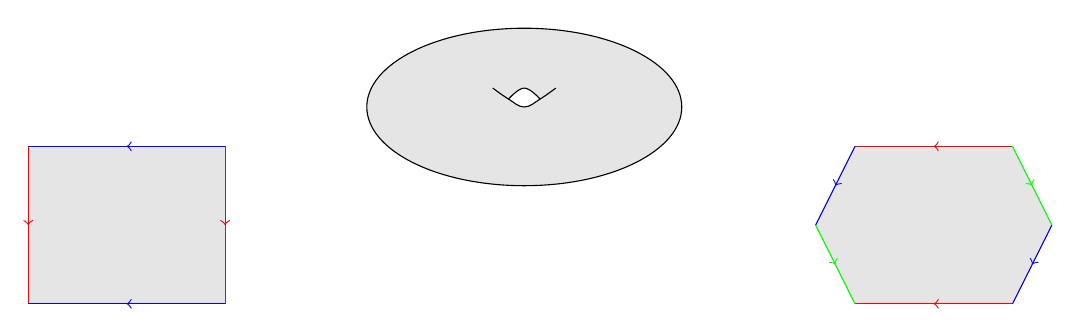
\begin{tikzpicture}
\tikzset{ ->-/.style={decoration={markings, mark=at position .5 with {\arrow{>}}}, postaction={decorate}}}
\draw[fill=gray!20]  (-1.2,-0.5) ellipse (2 and 1);

 \begin{scope}[shift={(2.2,-0.6)}]
    
    \fill[white]  plot[smooth, tension=0.7] coordinates { (-3.6,0.2) (-3.4,0.1) (-3.2,0.2) }  plot[smooth, tension=0.7] coordinates {(-3.6,0.2) (-3.4,0.34) (-3.2,0.2)};
    
    \draw  plot[smooth, tension=0.7] coordinates {(-3.8,0.34) (-3.6,0.2) (-3.4,0.1) (-3.2,0.2) (-3,0.34)};
    \draw  plot[smooth, tension=0.7] coordinates {(-3.6,0.2) (-3.4,0.34) (-3.2,0.2)};
    
    
    
    \end{scope}

\fill[gray!20]  (-7.5,-1) rectangle (-5,-3);
\fill[gray!20] (3,-1) -- (2.5,-2) -- (3,-3) -- (5,-3) -- (5.5,-2) -- (5,-1) -- cycle;

\draw[->-, red] (-5,-1) -- (-5,-3);
\draw[->-,red](-7.5,-1) -- (-7.5,-3);
\draw[->-, blue] (-5,-1) -- (-7.5,-1);
\draw[->-,blue] (-5,-3) -- (-7.5,-3);
\draw[->-, red] (5,-1) -- (3,-1);
\draw[->-,red] (5,-3) -- (3,-3);
\draw[->-,blue] (3,-1) -- (2.5,-2);
\draw[->-,blue] (5.5,-2) -- (5,-3);
\draw[->-,green] (5,-1) -- (5.5,-2);
\draw[->-,green] (2.5,-2) -- (3,-3);
\end{tikzpicture}

Heegaard diagrams are one way to produce a combinatorial presentation 3-manifold, for which there exist a nice set of moves between diagrams corresponding to the same manifold.

In the setting of surfaces, we have invariants associated to fundamental polygons (the genus, and orientability) which characterize the equivalence classes of fundamental polygons up to ``moves''.
The Heegaard-Floer cohomology is an invariant (constructed using techniques similar to Lagrangian intersection Floer theory) that we can associate to a Heegaard diagram.


%tag:0007
%label:art:heegaardDiagrams
%author:JeffHicks
%name:"Heegaard Diagrams:combinatorial descriptions of 3 manifolds"
%type:article


%label:"def:heegaardSplitting"
%author:JeffHicks
%name:"Heegaard splitting"
%type:"definition"
%indepth:art:heegaardDiagram
%example:exm:heegaardSplitting


    Let $M$ be a closed 3-manifold. A \emph{genus $g$} Heegaard splitting of $M$ is a decomposition
    \[M=U_1\cup_{\Sigma_g} U_2\]
    where $U_1, U_2$ are genus $g$ handlebodies along with an identification of their boundaries (the surface $\Sigma_g)$ with a diffeomorphism.

%parent:"def:heegaardSplitting"
%author:JeffHicks
%name:"Heegaard splitting"
%type:"example"
%indepth:art:heegaardDiagram
%label:"exm:heegaardSplitting"


    Consider the 3-sphere
    \[M=S^3=\left\{(x_0, x_1, x_2, x_3)\st x_i\in \RR, \sum_{i=1}^3 x_i^2=1.\right\}\]
    Consider the decomposition of this into two halves along the $z_0$ coordinate:
    \begin{align*}
        U_1=\{(x_0, x_1, x_2, x_3)\in S^3 \st x_0\leq 0\}&& U_2=\{(x_0, x_1, x_2, x_3)\in S^3 \st x_0\geq 0\}
    \end{align*}
    Then both $U_1, U_2$ are diffeomorphic to the 3-ball, and are glued together by their common boundary $S^2=\Sigma_0$. See \cref{fig:heegaardSplitting}.
    %parent:def:heegaardSplitting
%author:JeffHicks
%name:"Heegaard splitting for $S^3$"
%type:"figure"
%indepth:art:heegaardDiagram
%label:"fig:heegaardSplitting"
%parent:"exm:heegaardSplitting"
%caption:"After identifying $S^3\setminus \{(1, 0, 0, 0)\}$ with $\RR^3$ via stereographic projection, the Heegaard splitting of $S^3$ is given by taking the unit sphere, which decomposes the sphere into two $3$-balls. We also draw the meridinal line $(\cos(\theta), \sin(\theta), 0, 0)$."



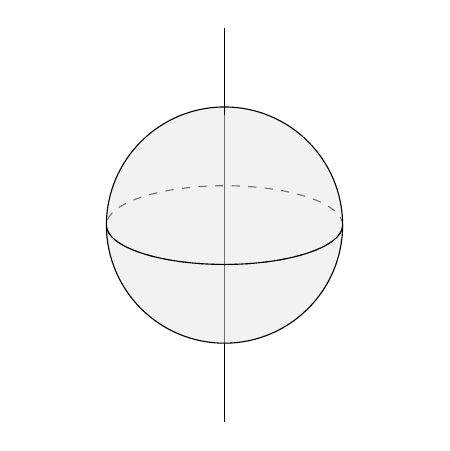
\begin{tikzpicture}
    \draw (-0.5,2) -- (-0.5,-3);
    \draw[dashed]  (-0.5,-0.5) ellipse (1.5 and 0.5);
    \draw[fill=gray!20, fill opacity=.5]  (-0.5,-0.5) ellipse (1.5 and 1.5);
    
    \draw (-0.5,2) -- (-0.5,0.9);
    
    \clip  (2,-0.5) rectangle (-3,-1.5);
    \draw  (-0.5,-0.5) ellipse (1.5 and 0.5);
    \end{tikzpicture}
    \label{exm:heegaardSplitting}

A handlebody is a 3-manifold $U$ with boundary with a collection disks $\{f_i: D^2\to U\}_{i=1}^g$ which are embedded and disjoint, so that $U\setminus \bigcup_{i=1}^g \Im(f_i)=D^3$. 
\input{lem_handleBodies}
%label:"prp:existenceOfHeegaardSplitting"
%author:JeffHicks
%name:"existence of Heegaard splitting"
%type:"proposition"



    Let $M$ be a closed 3-manifold. There exists a Heegaard splitting for $M$.
    \label{prp:existenceOfHeegaardSplitting}

%label:"proof:existenceOfHeegaardSplitting"
%author:JeffHicks
%name:"existence of Heegaard splitting"
%type:"proof"
%parent:prp:existenceOfHeegaardSplitting


    Let $f: M\to \RR$ be a self indexing Morse function. Consider the level set $f^{-1}(1.5)$. Because $1.5$ is not a critical value of $f$, this is a smooth surface $\Sigma_g\subset M$. Let $U_1=f^{-1}([0, 1.5])$ and let $U_2=f^{-1}([1.5, 3])$. By \cref{lem:handlebodies}, these are handlebodies.

To determine the data of a Heegaard splitting, one must specify the data of two fillings of $\Sigma_g$ by handlebodies. When the Heegaard splitting is determined by a self-indexing Morse function $f: M\to \RR$, we can use the critical points to determine the fillings $U_1$ and $U_2$ based on data contained in $\Sigma_g$. The filling $U_1$ is constructed by considering how the downward flow spaces of the critical points of $f|_{U_1}$ attach to the $\Sigma_g$. We may additionally assume  that $f$ has a unique maximum; then to determine the filling we only need to consider how $W^\downarrow(p)$ intersects $\Sigma_g$ for $\{p\in \Crit(f), \ind(p)=1\}$. Furthermore, there are $g$ such critical points which we enumerate as $\{p_i\}_{i=1}^g$. These downward flow spaces are 2-dimensional, so $\{\Sigma_g\cap W^\downarrow(p_i)\}_{i=1}^g$ gives $g$ disjoint cycles in $\Sigma_g$. We call these cycles 
\[\{\alpha_i\}_{i=1}^g:=\{ W^\downarrow(p_i)\cap \Sigma_g\}_{p_i\in \Crit(f), \ind(p_i)=1}\]
Similarly, we can consider the index 2 critical points of $f$, which are all contained in $U_2$, and look at their upward flow spaces
\[\{\beta\}_{i=1}^g:=\{ W^\uparrow(p_i)\cap \Sigma_g\}_{p_i\in \Crit(f), \ind(p_i)=1}.\]
%tag:0007
%label:def:heegaardDiagram
%author:JeffHicks
%name:"Heegaard diagram"
%type:definition


    A \emph{Heegaard diagram} is a triple $(\Sigma_g, \{\alpha_i\}_{i=1}^g, \{\beta_i\}_{i=1}^g$). Here, $\Sigma_g$ is a genus $g$ surface and $\{\alpha_i\}_{i=1}^g, \{\beta_i\}_{i=1}^g$ are collections of smooth 1-cycles in $\Sigma_g$ such that
    \begin{itemize}
         \item $\Sigma_g\setminus \{\alpha_i\}_{i=1}^g, \Sigma_g\setminus \{\beta_i\}_{i=1}^g$ are connected and;
         \item $\alpha_i\cap \alpha_j=\emptyset = \beta_i \cap \beta_j$ whenever $i\neq j$.
    \end{itemize}

We will usually write $\underline \alpha, \underline \beta$ for $\{\alpha_i\}_{i=1}^g, \{\beta_i\}_{i=1}^g$.
\input{exm_heegaardDiagram3sphere}
Every Heegaard diagram specifies a 3-manifold, however a single 3-manifold can have many different presentations with different Heegaard diagrams. We have already seen 2 different Heegaard diagrams for $S^3$ in \cref{exm:heegaardSplitting} and  \cref{exm:heegaardDiagram3sphere}. 
Therefore, if we are to study 3-manifolds via their Heegaard diagram, we need to understand when two diagrams give presentations of the same manifold. We first describe some operations which modify a Heegaard diagram, but produce the same 3-manifold. 
%label:def:heegaardStabilization
%author:JeffHicks
%name:"Heegaard stabilization"
%type:definition


    Let $(\Sigma_g, \{\alpha_i\}_{i=1}^g, \{\beta_i\}_{i=1}^g)$ be a Heegaard diagram. Let $p\in \Sigma_g$ be a point avoiding the cycles $\alpha_i, \beta_i$. The \emph{stabilization of $\Sigma_g$ at $p$} is the diagram $(\Sigma_g \#_p T^2, \{\alpha_i\}_{i=1}^{g+1}, \{\beta_i\}_{i=1}^{g+1})$ where $\alpha_{g+1}, \beta_{g+1}$ are the meridional and longitudinal classes of $T^2$.

%label:"rem:heegaardStabilizations"
%author:JeffHicks
%name:"Morse interpretation of Heegaard stabilization"
%type:"remark"
%parent:"def:heegaardStabilization"

One way to see that stabilization of a Heegaard diagram produces the same manifold comes from Morse theory. Consider $\Sigma_g$ as the level set of a self-indexing Morse function $f$. Suppose that we wanted to modify our Morse function to $\tilde f$ by adding in a pair of critical points $p, q$ so that $\ind(p)=1$ and $\ind(q)=2$. We imagine that the critical points would appear on opposite sides of $\Sigma_g$, and be connected by a single flow line. Furthermore, $\tilde \Sigma_{g+1}=\tilde f(1.5)$, the new level set, would be of genus $g+1$. By applying surgery along either the attaching circles $W^\downarrow(p)\cap \tilde \Sigma_{g+1}$ or $W^\uparrow(q)\cap \tilde \Sigma_{g+1}$, we obtain $\Sigma_g$. See \cref{fig:heegaardStabilization}.
%label:"fig:heegaardStabilization"
%author:JeffHicks
%name:"rounding corner in Polterovich surgery"
%type:"figure"
%parent:"thm_roundingCorner"
%caption:"From the perspective of Morse theory, stabilization comes from the creation of a pair of cancelling critical points."



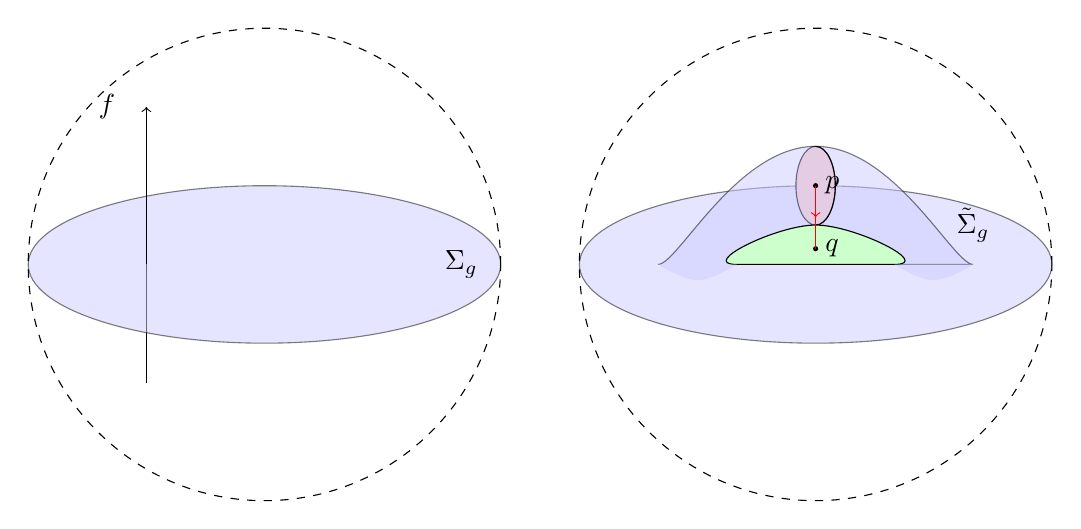
\begin{tikzpicture}
    \draw (-4,-1) -- (-4,0.5) ;
    \draw[opacity=.5,fill= blue!20]  (-2.5,0.5) ellipse (3 and 1);
    \draw[opacity=.5, fill=blue!20]   (4.5,0.5) node (v1) {} ellipse (3 and 1);
    \draw (6,-2);
    \draw[->](-4,0.5) -- (-4,2.5);
    \node at (-4.5,2.5) {$f$};
    \node at (0,0.5) {$\Sigma_g$};
    \draw[dashed]  (-2.5,0.5) ellipse (3 and 3);
    \draw[dashed]  (v1) ellipse (3 and 3);
    \draw[fill=red!20]  (4.5,1.5) ellipse (0.25 and 0.5);
    \draw[opacity=.5, fill=blue!20] (2.5,0.5) .. controls (2.75,0.5) and (3.5,2) .. (4.5,2) .. controls (5.5,2) and (6.25,0.5) .. (6.5,0.5) .. controls (6.25,0.5) and (6.25,0.5) .. (5.5,0.5) .. controls (5.75,0.5) and (5,1) .. (4.5,1) .. controls (4,1) and (3.25,0.5) .. (3.5,0.5);
    
    \node[right] at (4.5,1.5) {$p$};
    \node[fill=black, circle, scale=.2] at (4.5,1.5) {};
    \begin{scope}[]
    
    \clip  (5,1) rectangle (4.5,2);
    \draw  (4.5,1.5) ellipse (0.25 and 0.5);
    \end{scope}
    
    
    
    \draw[fill=green!20] (3.5,0.5) .. controls (3,0.5) and (4,1) .. (4.5,1) .. controls (5,1) and (6,0.5) .. (5.5,0.5)--cycle;
    \node[right] at (4.5,0.7) {$q$};
    \node[circle, fill=black, scale=.2] at (4.5,0.7) {};
    
    \begin{scope}[]
    
    \fill[opacity=.5, fill=blue!20]  plot[smooth, tension=.7] coordinates {(2.5,0.5) (3,0.3) (3.5,0.5)};
    
    \end{scope}\begin{scope}[shift={(3,0)}]
    
    \fill[opacity=0.5, fill=blue!20]  plot[smooth, tension=0.7] coordinates {(2.5,0.5) (3,0.3) (3.5,0.5)};
    
    \end{scope}\node at (6.5,1) {$\tilde \Sigma_g$};
    
    \draw[red,->] (4.5,1.5) -- (4.5,1.1);
    \draw[red] (4.5,1.1) -- (4.5,0.7);
    \end{tikzpicture}

%tag:0007
%label:def:heegaardMoves
%author:JeffHicks
%name:"Heegaard moves"
%type:definition


    Let $(\Sigma_g,\{\alpha_i\}_{i=1}^g, \{\beta_i\}_{i=1}^g)$ be a Heegaard diagram. We say that another diagram $(\Sigma_g,\{\alpha_i'\}_{i=1}^{g}, \{\beta_i'\}_{i=1}^{g})$ is related to $(\Sigma_g,\{\alpha_i\}_{i=1}^g, \{\beta_i\}_{i=1}^g)$ by an
    \begin{itemize}
        \item isotopy if the sets $\{\alpha_i\}_{i=1}^g, \{\alpha_i'\}^g$ are isotopic in $\Sigma_g$, or  $\{\beta_i\}_{i=1}^g, \{\beta_i'\}^g$ are isotopic in $\Sigma_g$.
        \item handle slide if $\alpha_i=\alpha_{i'}$ for $i\neq g$, and the curves $\alpha_{g-1}, \alpha_g, \alpha_g'$ bound a pair of pants in $\Sigma_g$ disjoint from $\{\alpha_i\}_{i=1}^{g-2}$ (or similarly for the $\beta_i$). See \cref{fig:handleslide}
    \end{itemize}


%label:"fig:handleslide"
%author:JeffHicks
%name:"handleslide"
%type:"figure"
%parent:def:heegaardMoves
%caption:"The cycles \(\alpha_{g-1}, \alpha_g\)and \(\alpha_g'\) are related by handleslide"



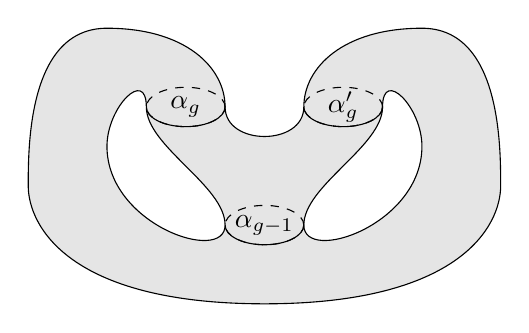
\begin{tikzpicture}





    \draw[fill=gray!20] (-0.5,1.5) .. controls (-1.5,1.5) and (-1.5,0) .. (-1.5,-0.5) .. controls (-1.5,-1) and (-1,-2) .. (1.5,-2) .. controls (4,-2) and  (4.5,-1) .. (4.5,-0.5) .. controls (4.5,0) and (4.5,1.5) .. (3.5,1.5) .. controls (2.5,1.5) and (2,1) .. (2,0.5) .. controls (2,0) and (1,0) .. (1,0.5) .. controls (1,1) and (0.5,1.5) .. (-0.5,1.5);
    \begin{scope}[]
    \draw[fill=white] (0,0.5) .. controls (0,1) and (-0.5,0.5) .. (-0.5,0) .. controls (-0.5,-1) and (1,-1.5) .. (1,-1) .. controls (1,-0.5) and (0,0) .. (0,0.5);
    
    \end{scope}
    \begin{scope}[xscale=-1, shift={(-3,0)}]
    \draw[fill=white] (0,0.5) .. controls (0,1) and (-0.5,0.5) .. (-0.5,0) .. controls (-0.5,-1) and (1,-1.5) .. (1,-1) .. controls (1,-0.5) and (0,0) .. (0,0.5);
    
    \end{scope}
    
    
    \begin{scope}[shift={(1,1.5)}]
    \draw[dashed]  (1.5,-1) ellipse (0.5 and 0.25);
    \clip  (2,-1) rectangle (1,-1.75);
    \draw  (1.5,-1) ellipse (0.5 and 0.25);
    \end{scope}
    
    
    \begin{scope}[shift={(0,0)}]
    \draw[dashed]  (1.5,-1) ellipse (0.5 and 0.25);
    \clip  (2,-1) rectangle (1,-1.75);
    \draw  (1.5,-1) ellipse (0.5 and 0.25);
    \end{scope}
    
    
    \begin{scope}[shift={(-1,1.5)}]
    \draw[dashed]  (1.5,-1) ellipse (0.5 and 0.25);
    \clip  (2,-1) rectangle (1,-1.75);
    \draw  (1.5,-1) ellipse (0.5 and 0.25);
    \end{scope}
    
    \node at (1.5,-1) {$\alpha_{g-1}$};
    \node at (0.5,0.5) {$\alpha_g$};
    \node at (2.5,0.5) {$\alpha_g'$};
    \end{tikzpicture}
%label:"thm:heegaardMoves"
%author:JeffHicks
%name:"Heegaard moves generate equivalences"
%type:"theorem"
%source:"singer1933three"


    \label{thm:heegaardMoves}
    Suppose that $(\Sigma_g,\underline \alpha, \underline \beta)$ and $(\Sigma_{g'},\underline \alpha', \underline \beta')$ are Heegaard diagrams for $M$. There exist a sequence of Heegaard moves and stabilizations taking one to the other. 

It follows that in order to construct 3-manifold invariants, one needs to find  quantities associated to the Heegaard diagram which are invariant under stabilizations, isotopies, and handles slides. Heegaard-Floer cohomology provides such an invariant.
%tag:0007
%label:"art:heegaardFloerConstruction"
%author:JeffHicks
%name:"Construction of Heegaard Floer cohomology"
%type:"article"


We will associate to the data of a Heegaard diagram $(\Sigma_g, \{\alpha_i\}_{i=1}^g, \{\beta_i\}_{i=1}^g)$ a pair of Lagrangian submanifolds in the $g$-th symmetric product of $\Sigma_g$, and compute a version of their Lagrangian intersection Floer cohomology. 
%tag:0007
%label:art:heegaardFloerConstruction
%author:JeffHicks
%name:"Symmetric products in symplectic geometry "
%type:article

%label:"def:symmetricProduct"
%author:JeffHicks
%name:"symmetric product"
%type:"definition"


    Let $X$ be a topological space. The $k$-symmetric product is the space 
    \[\Sym^k(X):=X^k/S_k\]
    where $S_n$ is the symmetric group on $k$-generators which acts by permutation on the factors of $\Sym^k(X)$.

In general, the symmetric product of a manifold does not have the structure of a manifold (as the symmetric group does not act freely on the diagonal). However, when $X$ is a complex curve (real surface) we are able to equip $\Sym^k(X)$ with the structure of a smooth complex manifold.
%label:"thm:symmetricProductOfSurfaceIsSmooth"
%author:JeffHicks
%name:"symmetric product of surfaces is smooth"
%type:"theorem"


    Let $(\Sigma, \jmath)$ be a complex curve. Then $\Sym^n(\Sigma)$ is a complex manifold, and the map $\Sigma^k\to \Sym^k(\Sigma)$ is holomorphic.

%label:"prf:symmetricProductOfSurfaceIsSmooth"
%author:JeffHicks
%name:"proof that the symmetric product of surfaces is smooth"
%type:"proof"
%parent:"thm:symmetricProductOfSurfaceIsSmooth"


    We prove this in the setting where $\Sigma=\CC$ (this will serve as a local model for the general setting). 
    Consider the space of polynomials of degree $n$ with leading coefficient 1, 
    \[\CC[z]_n:=\{z^n+a_{n-1}z^{n-1}+\cdots + a_1z+a_0\st a_i\in \CC\}\]
    There is a map from $\CC[z]_n\to \Sym^n(\CC)$ which sends each polynomial to its (unordered) set of zeros. This map is a bijection as every set of $n$ points (with possible repetition) in $\CC$ uniquely determines a degree $n$ polynomial with leading coefficient 1.
    The complex structure comes from identifying $\CC[z]_n = \CC^n$.

%label:"exm_symmetricProductOfP1"
%name:"$A_\infty$ Yoneda module"
%type:"example"



    We identify the symmetric product $\Sym^2(\CP^1)$ with $\CP^2$. To each point in $\CP^2$ we can associate a degree 2 homogenous polynomial in 2-variables:
    \[(z_0:z_1:z_2)\mapsto z_0 s^2 + z_1 st + z_2 t^2\]
    We then factor the polynomial as
    \[( z_0 s^2 + z_1 st + z_2 t^2)=(y_0 s + y_1 t)\cdot (x_0 s + x_1 t)\]
    This gives us a bijection between the points of $\CP^2$ and $\Sym^2(\CP^1)$. 
    \[(z_0:z_1:z_2)\mapsto [(x_0:x_1), (y_0,y_1)]\]
    
    Observe that the moment polytope of $\CP^1\times \CP^1$ is the square given by 
    \[\text{Convex Hull}((0,0), (0,1), (1, 0), (1, 1)),\]
    while the moment polytope of $\CP^2$ is given by the convex hull of
    \[\text{Convex Hull}((0,0), (0,1), (1,1)).\]
    There is map from the first moment polytope to the second (given by ``folding'' along the diagonal) which is 2-1 away from the diagonal (and 1-1 along the diagonal), allowing us to see the symmetric product on the level of moment polytopes.    

While $\Sym^k(\Sigma)$ is a complex manifold it \emph{does not} come with a canonical choice of symplectic structure, so we are leaving some of the tools that we use to study Lagrangian intersection Floer cohomology behind. 
%label:"con:heegaardFloer"
%author:JeffHicks
%name:"construction of Heegaard Floer complex"
%type:"construction"

Let $(\Sigma_g, \underline{\alpha}, \underline{\beta})$ be a Heegaard diagram. Let $X=\Sym^g(\Sigma_g)$. Consider the submanifolds of $X$
\begin{align*}
    L_{\underline \alpha}:=\{[(z_1, \ldots, z_g)]\in X\st z_i\in \alpha_i\} && 
    L_{\underline \beta}:=\{[(z_1, \ldots, z_g)]\in X\st z_i\in \beta_i\}
\end{align*}
Since the $\alpha_i$ are disjoint from one another, this gives a smooth submanifold whose topology is $T^g$. Furthermore, since each of the $\alpha_i$ is a real subspace of $\Sigma_g$, the submanifold $L_\alpha$ is a real submanifold of $\Sigma_g$. A similar statement holds for $L_\beta$. \Cite{perutz2008handleslide} shows that $\Sym^g(\Sigma_g)$ can be equipped with a symplectic form which makes $L_{\underline \alpha},L_{\underline \beta}$ Lagrangian submanifolds. 

We wish to define the Heegaard-Floer cohomology as the Lagrangian intersection Floer cohomology of $L_{\underline \alpha},L_{\underline \beta}$. However, this is not an invariant of Heegaard diagrams --- note that isotopies of Heegaard diagrams give isotopies of Lagrangian submanifolds, while Lagrangian intersection Floer cohomology is only invariant under \emph{Hamiltonian isotopies} of Lagrangian submanifolds. We given an example exhibiting some of the problems with this preliminary approach.

%tag:0007
%label:exm:nonadmissibleHeegaardDiagram
%author:JeffHicks
%name:"Heegaard diagrams for $S^2\times S^1$"
%type:example


    We look at the example of $M=S^2\times S^1$. Observe that $S^2=D^2\cup_{S^1} D^2$, so we can write $M=D^2\times S^1 \cup_{\Sigma_1} D^2\times S^1$. 
    The Heegaard diagram $(\Sigma_1, \alpha, \beta)$ consists of a torus with two meridional cycles. 
    \input{fig_nonAdmissibleHeegaardDiagram}
    If the diagram is chosen so that $\alpha, \beta$ are disjoint, then the Lagrangian intersection Floer cohomology $\HF(\alpha, \beta)$ vanishes.
    \input{fig_admissibleHeegaardDiagram}
    However, if the diagram is chosen so that $\alpha, \beta'$ intersect transversely, the Lagrangian intersection Floer cohomology (with $\ZZ/2\ZZ$ coefficients) is $\ZZ/2\ZZ\oplus \ZZ/2\ZZ$. Note that $\beta'$ can be chosen so that it is Hamiltonian isotopic to $\beta$.
    
    The discrepancy between these two answers comes from the non-convergence of the homotopy between the composition of continuation maps  $f\circ g:\CF(\alpha, \beta')\to \CF(\alpha, \beta) \to \CF(\alpha, \beta')$ and $\id: \CF(\alpha, \beta')$ over $\ZZ/2\ZZ$ coefficients. The presence of an annulus between $\alpha, \beta$ is the culprit for the non-convergence.

    If one instead chooses to use Novikov (instead of $\ZZ/2\ZZ$ coefficients) one can obtain a 

    To rule out this phenomenon, we only look at strips which avoid the marked point $z$, and will impose a criterion (admissible Heegaard diagrams) which will, in this setting, preclude the existence of annuli disjoint from the marked point $z$.  In general, the admissibility criterion will limit us to configurations of cycles for which the number of holomorphic strips contributing to the Floer differential is finite.




We desire the best of both worlds: invariance under Lagrangian isotopies, and convergence. In \cref{exm:nonadmissibleHeegaardDiagram} this can be achieved by only looking at strips which avoid the marked point $z$. When this marked point is chosen well, we will obtain a criterion (admissible Heegaard diagrams) which precludes the existence of annuli disjoint from the marked point $z$.  In general, the admissibility criterion will limit us to configurations of cycles for which the number of holomorphic strips contributing to the Floer differential is finite.

The marked point is introduced by slightly generalizing our definition of a Heegaard diagram. 
%tag:0007
%label:def:basedHeegaardDiagram
%author:JeffHicks
%name:"based Heegaard diagram"
%type:definition


    A \emph{based Heegaard diagram}  $(\Sigma_g, \underline \alpha, \underline \beta, z)$ is a Heegaard diagram $(\Sigma_g, \underline \alpha, \underline \beta)$ along with a choice of point $z$ disjoint from the cycles $\underline \alpha, \underline \beta$.
    \label{def:basedHeegaardDiagram}

A similar theorem to \cref{thm:heegaardMoves} holds for based Heegaard diagrams.
As a vector space, the Heegaard Floer cohomology of the based Heegaard diagram $(\Sigma,\underline{\alpha}, \underline{\beta},z)$ is
\[\HeF(\Sigma, \underline{\alpha}, \underline{\beta},z):=\bigoplus_{x\in L_{\underline \alpha}\cap L_{\underline{\beta}}} \ZZ/2\ZZ\langle x\rangle.\]
The differential is defined in a manner similar to the Lagrangian intersection Floer cohomology, but we will need to overcome the following difficulties.

\begin{itemize}
    \item Gromov-Compactness: Observe that this is defined over $\ZZ/2\ZZ$ coefficients. In general, when we look at the strips connecting two points $x, y$, we are only guaranteed compactness of the moduli space of pseudoholomorphic strips which have bounded energy. To get around this problem --- when strips from $x$ to $y$ have possibly unbounded energy --- we would employ Novikov coefficients in Lagrangian intersection Floer cohomology. Here, we do not use such a coefficient ring. 
    \item  If we treat $X$ as a symplectic manifold, the Lagrangian submanifolds $L_{\underline \alpha}, L_{\underline \beta}$ are not tautologically unobstructed (i.e. $\omega(\pi_2(X, L))\neq 0$). We therefore must rule out disk and sphere bubbling to show that the differential squares to zero.
\end{itemize}

The choice of base point defines a subset $Y_z\subset X$ given by  
\[ Y_z:=\{[(z, z_2, \ldots, z_g)] \st z_i\in \Sigma_g\} \subset X\]
which is disjoint from $L_{\underline \alpha}\cup L_{\underline \beta}$. Both issues above can be avoided by only looking at strips which are disjoint from $Y_z$.

For $x, y\in L_{\underline \alpha}\cap L_{\underline \beta}$ let $\mathcal M(x, y)$ denote the moduli space of holomorphic strips with boundary on $L_{\underline \alpha}\cup L_{\underline \beta}$, and ends limiting to $x$ and $y$. Let $\mathcal M(x, y)_{z=0}^0$ be the zero-dimensional component of $\mathcal M(x, y)$ consisting of strips which are disjoint from $Y_z$. The differential of Heegaard Floer cohomology is defined by the structure coefficients
\[\langle d_zx , y \rangle = \#\mathcal M(x, y)_{z=0}^0.\]
The following lemmas rule out the presence of disk and sphere bubbling.
%label:lem:heegaardNoSpheres
%author:JeffHicks
%name:"sphere bubbling in Heegaard differential"
%type:lemma


    Suppose that $g>2$. Then $\pi_2(\Sym^g(\Sigma_g))=\ZZ$. The generator of this group intersects $Y_z$.

%label:lem:heegaardNoDisks
%author:JeffHicks
%name:"disk bubbling in Heegaard differential"
%type:lemma



    Suppose that $u: D^2\to L_\alpha$ is a holomorphic disk. Then the image of $u$ intersects $Y_z$.

Provided that we can show that $(d_z)^2=0$, the Heegaard-Floer cohomology is defined to be the homology of the chain complex
\[\HHeF(M):= H^\bullet(\HeF(\Sigma, \underline \alpha, \underline \beta ,z), d_z).\]
As a result of these two lemmas, our restriction to counting disks which \emph{do not} pass through $Y_z$ gives us moduli spaces whose compactifications, if defined, would be free from disk and sphere bubbling. 

However, it remains to show that we have Gromov compactness.


%tag:0007
%label:"art:convergenceHeegaardFloer"
%author:JeffHicks
%name:"admissibility and convergence"
%type:"exposition"

In order to obtain a replacement for the symplectic form providing a bound on the energy of holomorphic strips, we need to work a little bit harder. The key insight is that there is a dictionary between holomorphic strips in the symmetric product and maps from more-complicated domains to the surface.

%label:prp:intersectionsInSymmetricProducts
%author:JeffHicks
%name:"intersection of Lagrangians in symmetric product"
%type:proposition


    Let $\underline \alpha = \{\alpha_i\}_{i=1}^g, \underline \beta = \{\beta_i\}_{i=1}^g$ be $g$-tuples of disjoint curves in $\Sigma_g$, so that $\alpha_i\cap \beta_j$ intersect transversely. Then there is a bijection between
    \[L_{\underline \alpha}\cap L_{\underline \beta} = \{(x_1, \ldots, x_g)\;|\; x_i\neq x_j, x_i \in \underline \alpha \cap \underline \beta.\}\]

This means that we can understand the intersections between our Lagrangians $L_{\underline \alpha}, L_{\underline \beta}$ in terms of the intersections between the collection of cycles. Remarkably, we can also understand the holomorphic strips between the intersections points by looking at data on $\Sigma_g$. 
%label:"thm:stripsInSymmetricProducts"
%author:JeffHicks
%name:"strips in the symmetric product"
%type:"theorem"


    Given a holomorphic strip $u\in \mathcal M(x, y)$ there exists a $g$-branched cover
    $\pi: \hat D\to D$ 
    and a holomorphic map from $\hat u: \hat D \to \Sigma_g$ so that for all $z\in D$, 
    \[u(z)=[(\hat u(z_1), \hat u(z_2), \cdots , \hat u(z_g)])\]
    where $\{z_1, \ldots, z_g\}\in \pi^{-1}(z)$.

With this relation, we can ``by hand'' rule out the kinds of problematic disks which would interfere with the arguments of Gromov-compactness.
%label:"def:heegaardDomain"
%author:JeffHicks
%name:"Heegaard domain"
%type:"definition"


    A \emph{Heegaard domain} (or simply domain) is a formal linear combination of the connected components of $\Sigma\setminus (\underline \alpha\cup \underline \beta)$.

%label:"def:periodicHeegaardDomain"
%author:JeffHicks
%name:"periodic Heegaard domain"
%type:"definition"

    A domain is \emph{periodic} if its boundary can be written as a sum of the cycles in $\underline \alpha, \underline \beta$ and it has no intersection with the marked point $z$.

    Every periodic domain can be represented by a surface with boundary $\hat D\to \Sigma$, thus every periodic domain $\mathcal D$ gives a homology class $H_2(M; \ZZ)$ by gluing the attaching disks associated to each of the $\alpha_i, \beta_j$ to the appropriate boundaries in $\hat D$. We call this homology class $H(\mathcal D)$.
%label:def:weaklyAdmissibleHeegaardDiagram
%author:JeffHicks
%name:"weakly admissible Heegaard diagram"
%type:definition


    A pointed Heegaard diagram is \emph{weakly admissible} if for a spin-c structure $s$ if for every non-trivial periodic domain $\mathcal D$ with 
    \[\langle c_1(s), H(\mathcal D)\rangle = 0\]
    $\mathcal D$ has both positive and negative coefficients.

The following lemma may give us some intuition for where the admissibility condition enters into the definition of Heegaard-Floer cohomology.
%label:"lem:heegaardAdmissibleZeroArea"
%author:JeffHicks
%name:"zero area periodic domains"
%type:"lemma"
%source:ozsvath2004holomorphic
%sourceDetail:"lemma 4.12"

    The following are equivalent:
    \begin{itemize}
        \item $(\Sigma_g, \underline \alpha, \underline \beta)$ is admissible for all $\Spinc$ structures
        \item There exists a symplectic form on $\Sigma$ so that every periodic domain as total signed area 0. 
    \end{itemize}

%label:"lem:heegaardAdmissibleFiniteStrips"
%author:JeffHicks
%name:"finitely many strips in Heegaard differential"
%type:"lemma"
%source:"ozsvath2004holomorphic"
%sourceDetail:"Lemma 4.14"


    Suppose that $(\Sigma, \alpha, \beta, z)$ is a weakly admissible Heegaard diagram. There are only finite many $\phi\in \pi_2(x, y)$ with $\mu(\phi)-j, n_z(\phi)=k, \mathcal D(\phi)\geq 0$.

This shows that the symplectic energy of the holomorphic strips that we consider in the definition of the differential $d_z$ is bounded. 


%tag:0007
%label:"art:invarianceOfHeegaardFloer"
%author:JeffHicks
%name:"invariance of Heegaard-Floer cohomology"
%type:"article"

%label:"thm:invarianceOfHeegaardFloer"
%author:JeffHicks
%name:"Heegaard moves generate equivalences"
%type:"theorem"


    Suppose that $(\Sigma_g,\underline \alpha, \underline \beta,z)$ and $(\Sigma_{g'},\underline \alpha', \underline \beta',z')$ are pointed admissible Heegaard diagrams for $M$. Then
    \[\HHeF(\Sigma, \underline{\alpha}, \underline{\beta},z)\cong\HHeF(\Sigma, \underline{\alpha}, \underline{\beta},z).\]

The proof of this theorem is beyond the scope of these notes. However, we can outline some of the steps in the proof. 
\begin{enumerate}
    \item Show that a similar theorem to \cref{thm:heegaardMoves} holds for pointed Heegaard diagrams.
    \item Invariance of $\HHeF(\Sigma_g, \underline \alpha, \underline \beta, z)$ under isotopies of almost complex structure. 
    \item Invariariance of $\HHeF(\Sigma_g,\underline \alpha, \underline \beta,z)$ under isotopies which do not create/destroy critical points. This can be reduced to the previous step by pulling back the almost complex structure along the isotopy.
    \item  Invariariance of $\HHeF(\Sigma_g,\underline \alpha, \underline \beta,z)$ under isotopies which do not create/destroy critical points: these isotopies can always be taken to be Hamiltonian isotopies of the Lagrangian $L_{\underline \alpha}$. 
    \item Invariance of $\HHeF(\Sigma_g,\underline \alpha, \underline \beta,z)$ under stabilizations: see \cref{exr:invarianceOfHHF}.
    \item Invariance of $\HHeF(\Sigma_g,\underline \alpha, \underline \beta,z)$: by far, the trickiest portion of the proof. This requires looking at the product structure on Lagrangian intersection Floer cohomology.
\end{enumerate}
%label:"art:heegaardFloerExercises"
%author:JeffHicks
%name:"Exercises"
%parent:""art:heegaardFloer""
%type:"article"

These exercises were curated by Fraser Binns. 
\label{art:heegaardFloerExercises}

%label:"exr:sym2s1"
%type:"exercise"
%name:"Symmetric Product of $S^1$"


     What is $\Sym^2(S^1)$?


%label:"exr:homologyFromHeegaardDiagram"
%type:"exercise"
%name:"homology from Heegaard Diagram"


    Let $(\Sigma, \{\alpha_i\}_{i=1}^g, \{\beta_i\}_{i=1}^g)$ be a Heegaard diagram for $M$.. Let $A$ be the $g\times g$ matrix whose entries over $\ZZ/2\ZZ$ given by  
    \[a_{ij}=\alpha_{i}\cap \beta_j \text{mod} 2.\] 
    Given the matrix $A$, compute $H^\bullet(M, \ZZ/2\ZZ)$.


%label:"exr:homologyClassOfWhitneyDisk"
%type:"exercise"
%name:"homology classes of Whitney disk boundaries"


    \begin{enumerate}
            \item    Let $\Sigma$ be a surface. Show that $H_1(\Sym^g(\Sigma))\cong H_1(\Sigma)$.
            \item    Show that $H_1(\Sym^g(\Sigma))/(H_1(T_\alpha)\oplus H_1(T_\beta)\cong H_1(\Sigma))/\langle\{\alpha_i,\beta_j\}_{i,j}\rangle$
             \item   What is the homology class of the boundary of a psuedoholomorphic disk?
    \end{enumerate}


%label:"exr:heegaardFloerLensSpace"
%type:"exercise"
%name:"Heegaard Floer cohomology of lens spaces"


        A \emph{Lens space} $L(p,q)$ can be defined as the $3$-manifold with a Heegaard splitting of genus 1, with an $\alpha$-curve given by a longitude of the the torus, and the $\beta$-curve in the class $(p, q)$. Use the above obstruction to compute $\widehat{HHF}^\bullet(L(p,q))$.
        %label:"fig:heegaardDiagramLensSpace"
%type:"figure"
%author:JeffHicks
%name:"Heegaard diagram for the Lens space $L(2,3)"
%caption:"The Heegaard diagram for the Lens space $L(2,3)$"

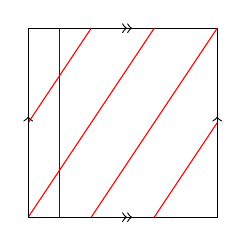
\begin{tikzpicture}[scale=2]

    \draw  (2.2,2.4) rectangle (3.4,1.2);
    \draw[blue] (2.4,2.4) -- (2.4,1.2);
    \draw[red] (2.2,1.2) -- (3,2.4) (3,1.2) -- (3.4,1.8) (2.2,1.8) -- (2.6,2.4) (2.6,1.2) -- (3.4,2.4);
    \draw[->] (2.2,1.2) -- (2.2,1.84);
\draw[->] (3.4,1.2) -- (3.4,1.84);
\draw[->>] (2.6,1.2) -- (2.86,1.2);
\draw[->>] (2.6,2.4) -- (2.86,2.4);
\end{tikzpicture}
    


%label:"exr:heegaardMoves"
%type:"exercise"
%name:"heegaard moves"


Compute the Heegaard Floer homology of the manifold with Heegaard splitting as shown, from the diagram. What is the manifold?
%parent:""exr:heegaardMoves""
%label:"fig:heegaardDiagramMystery"
%author:JeffHicks
%name:"Mystery Heegaard Diagram"
%type:"diagram"

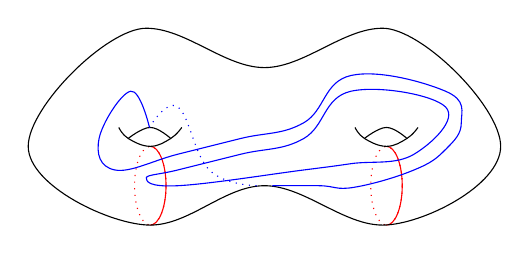
\begin{tikzpicture}


    \begin{scope}[shift={(-0.75,0)}]
    \draw[red,dotted]  (-1.2,-1) ellipse (0.2 and 0.5);
    \clip  (-0.8,-1.6) rectangle (-1.2,0);
    \draw[red]  (-1.2,-1) ellipse (0.2 and 0.5);
    \end{scope}
    
    
    \begin{scope}[shift={(2.25,0)}]
    \draw[red,dotted]  (-1.2,-1) ellipse (0.2 and 0.5);
    \clip  (-0.8,-1.6) rectangle (-1.2,0);
    \draw[red]  (-1.2,-1) ellipse (0.2 and 0.5);\end{scope}
    
    
     \begin{scope}[shift={(4.45,-0.6)}]
        
        \fill[white]  plot[smooth, tension=0.7] coordinates { (-3.68,0.2) (-3.4,0.1) (-3.14,0.2) }  plot[smooth, tension=0.7] coordinates {(-3.68,0.2) (-3.4,0.34) (-3.14,0.2)};
        
        \draw  plot[smooth, tension=0.7] coordinates {(-3.8,0.34) (-3.68,0.2) (-3.4,0.1) (-3.14,0.2) (-3,0.34)};
        \draw  plot[smooth, tension=0.7] coordinates {(-3.68,0.2) (-3.4,0.34) (-3.14,0.2)};
        
        
        
        \end{scope}
        
        
     \begin{scope}[shift={(1.45,-0.6)}]
        
        \fill[white]  plot[smooth, tension=0.7] coordinates { (-3.68,0.2) (-3.4,0.1) (-3.14,0.2) }  plot[smooth, tension=0.7] coordinates {(-3.68,0.2) (-3.4,0.34) (-3.14,0.2)};
        
        \draw  plot[smooth, tension=0.7] coordinates {(-3.8,0.34) (-3.68,0.2) (-3.4,0.1) (-3.14,0.2) (-3,0.34)};
        \draw  plot[smooth, tension=0.7] coordinates {(-3.68,0.2) (-3.4,0.34) (-3.14,0.2)};
        
        
        
        \end{scope}
        
        
    \draw[blue]  plot[smooth cycle, tension=.7] coordinates {(-1.6,-0.8) (-2,-0.9) (-1.6,-1) (0,-0.8) (0.6,-0.72) (1.4,-0.6) (1.8,0) (0.6,0.2) (0,-0.4) (-0.8,-0.6)};
    
    \draw (-2,1) .. controls (-2.5,1) and (-3.5,0) .. (-3.5,-0.5) .. controls (-3.5,-1) and (-2.45,-1.5) .. (-1.95,-1.5) .. controls (-1.45,-1.5) and (-1,-1) .. (-0.5,-1) .. controls (0,-1) and (0.5,-1.5) .. (1,-1.5) .. controls (1.5,-1.5) and (2.5,-1) .. (2.5,-0.5) .. controls (2.5,0) and (1.5,1) .. (1,1) .. controls (0.5,1) and (0,0.5) .. (-0.5,0.5) .. controls (-1,0.5) and (-1.5,1) .. (-2,1);
    \draw[blue]  plot[smooth, tension=.7] coordinates {(-1.96,-0.26) (-2.2,0.2) (-2.6,-0.4) (-2.4,-0.8) (-1.6,-0.6) (-0.8,-0.4) (0,-0.2) (0.6,0.4) (1.8,0.2) (2,-0.2) (1.8,-0.54) (1.4,-0.8) (0.64,-1.02) (0.2,-1) (-0.4,-1)};
    \draw[blue, dotted]  plot[smooth, tension=.7] coordinates {(-0.6,-1) (-1.2,-0.8) (-1.6,0) (-1.96,-0.26)};
    \end{tikzpicture}
    


%label:"exr:eulerCharacteristicOfHeegaardDiagrams"
%type:"exercise"
%name:"Euler characteristic of Heegaard diagrams"


     \begin{enumerate}
            \item Let $Y$ be a $3$-manifold with Heegaard splitting $(\Sigma,\mathbf{\alpha},\mathbf{\beta})$. Pick  orientations on $\Sigma,\alpha,\beta$. Explain how this induces a $\ZZ/2$ grading on $\widehat{HHF}^\bullet(Y)$.
            
            \item Let $Y$ be a rational homology sphere. Show that 
            \[\chi(\widehat{HHF}^\bullet(Y)):=\operatorname{rank}(\widehat{HHF}^\bullet_0(Y))-\operatorname{rank}(\widehat{HHF}^\bullet_1(Y))=|H_1(Y;\ZZ)|.\]
            
            \item A rational homology sphere (i.e. a 3 manifold with $H_*(Y)\cong H_*(S^3)$) is called an \emph{L-space}, if $\operatorname{rank}(\widehat{HHF}^\bullet(Y))$ is minimal in the sense that $\operatorname{rank}(\widehat{HHF}^\bullet(Y))=|H_1(Y)|$. Explain why Lens spaces are $L$-spaces
        \end{enumerate}


%label:"exr:invarianceOfHHF"
%type:"exercise"
%name:"invariance of Heegaard Floer cohomology"


        \begin{enumerate}
            \item Consider the ``decatigorification" of $\widehat{HHF}^\bullet$ given by the Euler characteristic as described in the previous question. Show that it is invariant under Heegaard moves. How might the proof of invariance of $\widehat{HHF}^\bullet$ differ?
        \item  Suppose $Y_1,Y_2$ are $3$-manifolds. How are $\widehat{HHF}^\bullet(Y_1\# Y_2),\widehat{HHF}^\bullet(Y_1),$ and $\widehat{HHF}^\bullet(Y_2)$ related?
    \item Show that $\widehat{HHF}^\bullet$ is invariant under stabilization and Hamiltonian isotopy in the sense that the resulting groups are isomorphic.
        \end{enumerate}

